\documentclass[11pt,a4paper]{article}
\usepackage[T1]{fontenc}
\usepackage[margin=2.3cm]{geometry}
\usepackage{amsmath,amssymb}
\usepackage{graphicx}
\usepackage[dvipsnames]{xcolor}
\usepackage{enumitem}
\usepackage[colorlinks=true,linkcolor=blue,urlcolor=blue]{hyperref}
\setlength{\parskip}{0.6em}
\setlength{\parindent}{0pt}
\begin{document}

\begin{center}{\LARGE\bfseries opendesalination}\\[0.4em]{\large Estimate the energy to turn seawater into drinking water, in three sessions.}\\[0.2em]\small PAN IIT OSS explainer \textbullet{} diploma / undergraduate to advanced undergraduate (levels 5-6)\end{center}

\section*{Why this exists}
Making fresh water from seawater takes a minimum amount of energy set by physics. This explainer follows the idea from the osmotic pressure of seawater to the least work of separation and a simulated reverse osmosis membrane, using only the van 't Hoff law, a salt balance and the rule that pressure times volume is energy.

\section*{The end goal}
Estimate the energy to turn seawater into drinking water: to know the physical floor (about 0.8 to 1.1 kWh per cubic metre), to see which design choices add to it, and to explain why real seawater plants use roughly 3 to 4 kWh per cubic metre. The same ideas apply to brackish water, wastewater reuse and every other membrane separation.

\section*{How the three sessions build up}
\begin{enumerate}[nosep]
\item \textbf{Session 1: Osmotic pressure and the minimum energy} (Level 1, conceptual interactive model, 60 min).
\item \textbf{Session 2: Recovery, brine and the least work} (Level 2, mathematical design model, 75 min).
\item \textbf{Session 3: Simulate a membrane module and validate it} (Level 3, simulation and validation, 90 min).
\end{enumerate}

\textit{All models are simplified educational models, not validated design tools. Never drink water from a home-made membrane or filter.}

\section{Session 1: Osmotic pressure and the minimum energy}

\subsection*{A. Real-world problem}
Chennai gets part of its drinking water from seawater plants on the coast at Minjur and Nemmeli. Pulling the salt out of the sea costs electricity, and electricity costs money and fuel. Is there a smallest possible energy bill for each cubic metre of fresh water, one that no clever machine, however good, can beat? And is it closer to the energy of boiling the water or to the energy of pumping it up a hill? (General education only: this is a simplified model, not a plant design method.)

\subsection*{B. Concept and theory}
A \textbf{semi-permeable membrane} lets water molecules through but holds back salt ions. Put pure water on one side and salt water on the other: water flows into the salty side by itself (\textbf{osmosis}), because mixing is the natural direction of change. The pressure you must apply on the salty side to stop that flow is the \textbf{osmotic pressure} pi. For dilute solutions it follows the van 't Hoff law pi = i c R T, which looks like the ideal gas law: each dissolved particle "pushes" like a gas molecule. Here c is the salt concentration in mol/m3, i is the number of particles each salt unit splits into (2 for NaCl: Na+ and Cl-) and T is the absolute temperature. Push harder than pi and water flows the other way, out of the salt water: this is \textbf{reverse osmosis} (RO). Pushing a volume V of water against a pressure P costs the work W = P V, and 1 kPa x 1 m3 = 1 kJ. So the least energy to take a small amount of fresh water out of a large amount of seawater is pi per cubic metre. Since 1 kWh = 3600 kJ, the minimum in kWh/m3 is pi (in kPa) / 3600.

\begin{itemize}[nosep]
\item M: molar mass of NaCl, 58.44 (g/mol)
\item c: molar concentration S / M x 1000 (mol/m3)
\item i: dissolved particles per salt unit (van 't Hoff factor), 2 for NaCl (no unit)
\item R: gas constant, 8.314 (J/(mol K))
\item T: absolute temperature (degrees C + 273.15) (K)
\item pi: osmotic pressure (kPa)
\item E\_min: least energy per m3 of fresh water (kWh/m3)
\end{itemize}

\begin{equation*}
c = \frac{S}{M}\times 1000
\end{equation*}

\begin{equation*}
\pi = i\,c\,R\,T
\end{equation*}

\begin{equation*}
W = P\,V,\qquad 1\ \mathrm{kPa}\times 1\ \mathrm{m^3} = 1\ \mathrm{kJ}
\end{equation*}

\begin{equation*}
E_{\min} = \frac{\pi\ [\mathrm{kPa}]}{3600}\ \ \mathrm{kWh/m^3}
\end{equation*}

\begin{center}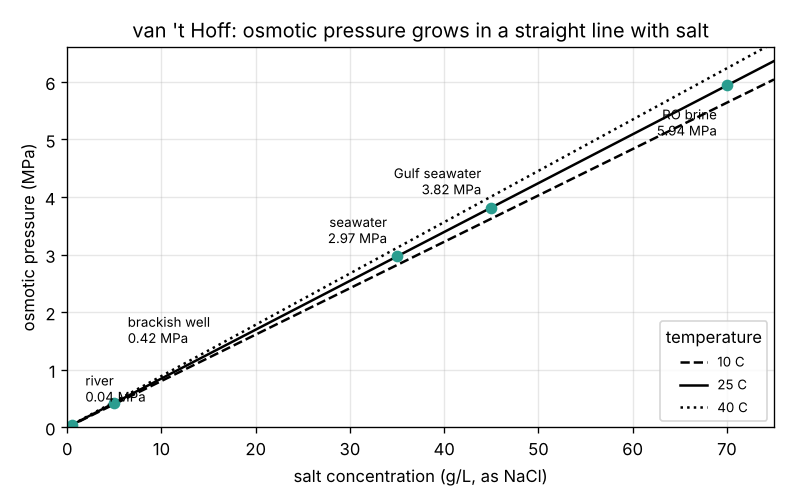
\includegraphics[width=0.85\linewidth]{figures/s01_osmotic_pressure.png}\\\small Osmotic pressure against salt concentration at three temperatures, with common waters marked.\end{center}

\subsection*{E. Worked example}
Seawater holds 35 g of salt per litre at 25 degrees C. Find its osmotic pressure, the least energy to take a small amount of fresh water out of it, and the height of a water column that would give the same pressure.
\begin{enumerate}[nosep]
\item Molar concentration: c = 35 / 58.44 x 1000 = 598.9 mol/m3.
\item Temperature in kelvin: T = 25 + 273.15 = 298.15 K.
\item Osmotic pressure: pi = 2 x 598.9 x 8.314 x 298.15 = 2 969 150 Pa = 2969 kPa (about 29.7 bar).
\item Minimum energy: 2969 kPa x 1 m3 = 2969 kJ per m3; divided by 3600 gives 0.825 kWh/m3.
\item Water column: h = P / (rho g) = 2 969 150 / (1000 x 9.81) = 303 m. Seawater pushes back as hard as a 300 m tower of water.
\end{enumerate}
\textbf{Answer.} pi = 2969 kPa, E\_min = 0.825 kWh/m3, equal to a water column of 303 m.

\subsection*{F. Questions}
\begin{enumerate}[nosep]
\item \textbf{Conceptual.} Why must there be a minimum energy for desalination, even with a perfect machine that has no friction and no leaks?
\item \textbf{Numerical.} A brackish well in Rajasthan has 5 g/L of salt at 25 degrees C. Find the osmotic pressure and the minimum energy, and compare with seawater.
\item \textbf{Graph and simulation interpretation.} In the osmotic pressure figure, the 40 degrees C line is above the 10 degrees C line. By what factor, and why is it not 40 / 10 = 4?
\item \textbf{Design and optimisation challenge.} Design: a coastal town of 50 000 people needs 100 litres per person per day from 35 g/L seawater at 25 degrees C. What is the minimum power (kW) that physics demands? A real plant uses 3.5 kWh/m3: what power does it need, and how many times the minimum is that?
\end{enumerate}

\section{Session 2: Recovery, brine and the least work}

\subsection*{A. Real-world problem}
A seawater plant does not take a tiny sip of fresh water. It pumps in seawater and takes out about 40 to 50 percent of it as fresh water; the rest leaves as brine, carrying all the salt. The brine is saltier than the sea and pushes back harder. How does the minimum energy grow when we take more of the feed? Why do plant designers settle near 50 percent, and how much does an energy recovery device save? (Simplified ideal model; not a plant design method.)

\subsection*{B. Concept and theory}
\textbf{Salt balance.} Feed a volume V with salt cf; take out a fraction r (the \textbf{recovery}) as fresh water. A perfect membrane keeps all the salt, so the brine (1 - r) V holds it all: cb = cf / (1 - r). Since pi is proportional to c, pi\_b = pi\_f / (1 - r). \textbf{Least work.} Picture a cylinder whose base is a membrane, holding seawater. Push the piston very slowly, always only just above the osmotic pressure of what is left. After a fraction x has gone, the pressure is pi(x) = pi\_f / (1 - x). As for a gas pushed by a pump, the work is the area under this curve; summing thin strips (an integral) gives pi\_f ln(1 / (1 - r)) per unit of feed, or W\_rev = pi\_f ln(1 / (1 - r)) / r per unit of fresh water. This is the reversible work: no process can use less (second law). As r tends to 0 it becomes pi\_f, the Session 1 answer. \textbf{One-stage plant.} A real plant is a steady flow, not a slow piston. The membrane only gives water while the push P is above the local osmotic pressure, and the last bit of membrane sees brine, so P must be at least pi\_b. With no energy recovery the pump lifts all the feed (1 / r per unit fresh water) to pi\_b: W = pi\_f / (r (1 - r)), smallest at r = 0.5 where it is 4 pi\_f. The brine leaves at high pressure; an \textbf{ERD} (a pressure exchanger) hands a share e of that pressure energy back to the incoming feed: W = pi\_f (1 - e (1 - r)) / (r (1 - r)). With e = 1 only pi\_b remains. \textbf{Stages.} n stages in series, each at its own outlet pressure, make a staircase under the curve pi(x); as n grows, the staircase hugs the curve and the work falls towards W\_rev.

\begin{itemize}[nosep]
\item cf, cb: salt in feed and brine (g/L)
\item pi\_f, pi\_b: osmotic pressure of feed and brine (kPa)
\item x: fraction of the feed removed so far (no unit)
\item W\_rev: least (reversible) work per m3 of fresh water (kWh/m3)
\item e: energy recovery device efficiency (no unit)
\item n: number of stages (no unit)
\end{itemize}

\begin{equation*}
c_b = \frac{c_f}{1-r},\qquad \pi_b = \frac{\pi_f}{1-r}
\end{equation*}

\begin{equation*}
W_{\mathrm{rev}} = \frac{1}{r}\int_0^r \frac{\pi_f}{1-x}\,dx = \frac{\pi_f}{r}\ln\frac{1}{1-r}
\end{equation*}

\begin{equation*}
W_{1} = \frac{\pi_f}{r(1-r)}\quad\text{(no ERD)},\qquad W_{1,e} = \frac{\pi_f\,[1-e(1-r)]}{r(1-r)}
\end{equation*}

\begin{equation*}
W_n = \frac{1}{r}\sum_{k=1}^{n}\frac{\pi_f}{1-k r/n}\,\frac{r}{n}\ \ \to\ W_{\mathrm{rev}}\ \text{as}\ n\to\infty
\end{equation*}

\begin{center}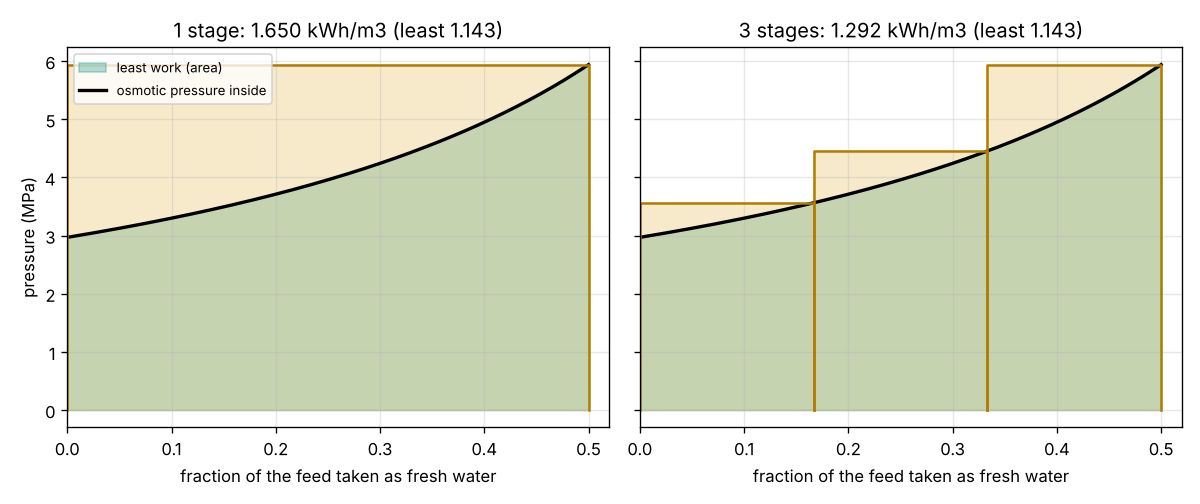
\includegraphics[width=0.85\linewidth]{figures/s02_pressure_staircase.png}\\\small Pressure staircase: the least work is the area under the curve; stages fit a staircase under it.\end{center}

\subsection*{E. Worked example}
Seawater (35 g/L, 25 degrees C, pi\_f = 2969 kPa) is desalinated at a recovery of 50 percent. Find the brine salt, the least work, and the energy of a one-stage plant without an ERD, with a 90 percent ERD and with a perfect ERD.
\begin{enumerate}[nosep]
\item Brine: cb = 35 / (1 - 0.5) = 70 g/L, so pi\_b = 2 x 2969 = 5938 kPa.
\item Least work: W\_rev = 2969 x ln(2) / 0.5 = 2969 x 0.6931 / 0.5 = 4116 kJ/m3 = 1.143 kWh/m3.
\item One stage, no ERD: W = 2969 / (0.5 x 0.5) = 11 877 kJ/m3 = 3.299 kWh/m3 (4 times pi\_f).
\item With a 90 percent ERD: W = 2969 x (1 - 0.9 x 0.5) / 0.25 = 6532 kJ/m3 = 1.815 kWh/m3.
\item With a perfect ERD: W = pi\_b = 5938 kJ/m3 = 1.650 kWh/m3, still 44 percent above the least work because one stage pushes everything at the brine pressure.
\end{enumerate}
\textbf{Answer.} cb = 70 g/L; W\_rev = 1.143 kWh/m3; one stage needs 3.30 (no ERD), 1.81 (90 percent ERD) and 1.65 kWh/m3 (perfect ERD).

\subsection*{F. Questions}
\begin{enumerate}[nosep]
\item \textbf{Conceptual.} Why does the least work grow with recovery, even though each cubic metre of fresh water is the same pure water?
\item \textbf{Numerical.} Find the least work at r = 0.4 for seawater (pi\_f = 2969 kPa) and the energy of one stage without an ERD at the same recovery. Check the units.
\item \textbf{Graph and simulation interpretation.} In the energy-against-recovery figure, why does the red curve (one stage, no ERD) have a minimum at 50 percent, while the least work curve keeps rising?
\item \textbf{Design and optimisation challenge.} Design: a plant must run at r = 0.5 on 35 g/L seawater. The pump can deliver at most 6900 kPa. Is one stage possible? Choose between 1 stage with a 95 percent ERD and 2 stages with a 95 percent ERD, and give the energy of each.
\end{enumerate}

\section{Session 3: Simulate a membrane module and validate it}

\subsection*{A. Real-world problem}
Session 2 assumed endless membrane area and perfect machines. A real seawater plant is built from pressure vessels, each holding about seven spiral-wound elements (roughly 260 m2 of membrane), fed by a high-pressure pump that wastes about 20 percent of its power and an energy recovery device (ERD) that returns most, not all, of the brine's push. The membrane also lets a little salt through. Can we simulate one vessel step by step, prove that the simulation obeys the balances and the limits we already know, and choose the feed pressure for a seawater plant? (A simplified teaching model, not a design tool.)

\subsection*{B. Concept and theory}
\textbf{Flux laws (solution-diffusion model).} Through each square metre of membrane the water flux is Jw = A (P - CP pi(c)): proportional to the push above the osmotic pressure at the membrane wall, and zero if the push is smaller. The salt flux is Js = B CP c: salt diffuses through in proportion to the salt at the wall. A and B are measured for each membrane. \textbf{Concentration polarisation.} Water leaves through the wall but salt stays, so salt piles up in a thin layer next to the wall; the wall is CP times saltier than the bulk (CP about 1.05 to 1.2), which raises the osmotic pressure that the pump must beat. \textbf{Marching.} Follow the feed channel from inlet to outlet. In a small area da, the water flow Q and the salt flow S drop by Jw da and Js da, and the bulk salt is c = S / Q. These two equations dQ/da = -Jw and dS/da = -Js are solved with the Runge-Kutta 4 method (four slope samples per step, weighted 1, 2, 2, 1). \textbf{Validation.} With B = 0 and CP = 1 the salt flow is fixed and dQ/da = -A (P - pi\_f Qf / Q) can be integrated by hand; the simulation must match it. No area can push the brine above P, so the recovery can never exceed 1 - pi\_f / P (the Session 2 limit), and the simulated energy can never be below the least work. \textbf{Energy.} The pump lifts all the feed to P with efficiency eta\_p; the ERD returns e of the brine's pressure energy P Qb: SEC = (P Qf / eta\_p - e P Qb) / Qp, in kJ per m3 (divide by 3600 for kWh/m3).

\begin{itemize}[nosep]
\item A: water permeability, 1e-5 (= 1 L/(m2 h bar)) (m3/(m2 h kPa))
\item B: salt permeability, 8e-5 (illustrative) (m3/(m2 h))
\item CP: concentration polarisation factor (no unit)
\item Jw, Js: water flux and salt flux (m3/(m2 h), kg/(m2 h))
\item Q, S: water flow and salt flow in the feed channel (m3/h, kg/h)
\item a: membrane area from the inlet (m2)
\item SEC: specific energy consumption per m3 of fresh water (kWh/m3)
\item eta\_p, e: pump efficiency and ERD efficiency (no unit)
\end{itemize}

\begin{equation*}
J_w = A\,\big(P - CP\,\pi(c)\big),\qquad J_s = B\,CP\,c
\end{equation*}

\begin{equation*}
\frac{dQ}{da} = -J_w,\qquad \frac{dS}{da} = -J_s,\qquad c = \frac{S}{Q}
\end{equation*}

\begin{equation*}
a(Q) = \frac{1}{A}\left[\frac{Q_f - Q}{P} + \frac{\pi_f Q_f}{P^2}\ln\frac{P Q_f - \pi_f Q_f}{P Q - \pi_f Q_f}\right]\quad (B = 0,\ CP = 1)
\end{equation*}

\begin{equation*}
r \le 1 - \frac{\pi_f}{P}
\end{equation*}

\begin{equation*}
\mathrm{SEC} = \frac{P\,Q_f/\eta_p - e\,P\,Q_b}{3600\,Q_p}
\end{equation*}

\begin{center}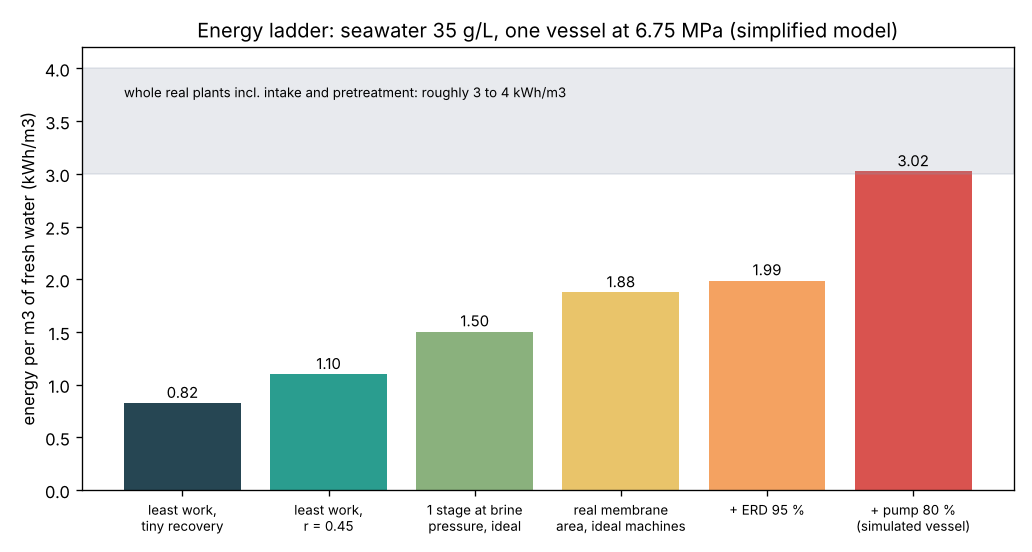
\includegraphics[width=0.85\linewidth]{figures/s03_energy_ladder.png}\\\small Energy ladder from the physical minimum to the simulated vessel.\end{center}

\subsection*{E. Worked example}
One vessel at P = 6000 kPa takes Qf = 12 m3/h of 35 g/L seawater (pi\_f = 2969 kPa, A = 1e-5 m3/(m2 h kPa), B = 0, CP = 1). How much membrane gives 30 percent recovery? Check the simulation, find the brine salt and the energy with an 80 percent pump and a 95 percent ERD.
\begin{enumerate}[nosep]
\item Flows: Qp = 0.3 x 12 = 3.6 m3/h, Qb = 12 - 3.6 = 8.4 m3/h. Constant k = pi\_f Qf = 2969 x 12 = 35 630 kPa m3/h.
\item Closed form: (Qf - Q) / P = 3.6 / 6000 = 0.000600; ln((6000 x 12 - 35 630) / (6000 x 8.4 - 35 630)) = ln(36 370 / 14 770) = ln(2.462) = 0.9011; k / P\textasciicircum{}2 x 0.9011 = 35 630 / 36 000 000 x 0.9011 = 0.000892. Area = (0.000600 + 0.000892) / 1e-5 = 149.2 m2.
\item RK4 march over 149.2 m2 in 400 steps gives recovery 0.300000 (difference below 1e-6). Brine: 35 / 0.7 = 50 g/L, so pi\_b = 4242 kPa, below P as it must be.
\item Energy: pump 6000 x 12 / 0.8 = 90 000 kJ/h; ERD returns 0.95 x 6000 x 8.4 = 47 880 kJ/h; net 42 120 kJ/h for 3.6 m3/h = 11 700 kJ/m3 = 3.25 kWh/m3.
\item Compare: least work at r = 0.3 is 0.98 kWh/m3; the vessel needs 3.3 times that.
\end{enumerate}
\textbf{Answer.} Area 149.2 m2, simulation agrees to 1e-6, brine 50 g/L, SEC 3.25 kWh/m3 (least work 0.98 kWh/m3).

\subsection*{F. Questions}
\begin{enumerate}[nosep]
\item \textbf{Conceptual.} Why does the water flux fall along the membrane, even though the feed pressure is the same everywhere?
\item \textbf{Numerical.} At the inlet of a vessel at 6000 kPa with 35 g/L feed and CP = 1.1, find the water flux in L per m2 per hour. What is it at the outlet if the brine there is 56 g/L?
\item \textbf{Graph and simulation interpretation.} In the energy ladder, which step costs the most energy, and which is a choice rather than a law of physics?
\item \textbf{Design and optimisation challenge.} Design: with the mini-project vessel, compare a pump of 80 percent and one of 85 percent at P = 6750 kPa. How much energy does the better pump save, and how much power is that for a 100 MLD (100 000 m3/day) plant?
\end{enumerate}

\section{Real-world mini-project}
\textbf{Choose the feed pressure for a seawater RO vessel.} A coastal plant uses vessels like the one above (260 m2, 12 m3/h feed, A = 1e-5, B = 8e-5, CP = 1.1, pump 80 percent, ERD 95 percent). The owner wants at least 45 percent recovery (to keep intake pumping and pretreatment small), fresh water below 500 mg/L of salt from the first pass, and the high-pressure piping is rated for 6900 kPa. Use \texttt{choose\_pressure} from Session 3 (steps of 250 kPa). These are illustrative values, not a membrane data sheet.

\section{The path ahead}
\begin{enumerate}[nosep]
\item \textbf{Session 4: Real seawater osmotic pressure.} An osmotic pressure function with an osmotic coefficient fitted to published seawater data, used in place of the ideal law in Sessions 1 to 3.
\item \textbf{Session 5: Pressure drop and a two-stage vessel train.} A pressure drop along the vessel inside \texttt{simulate\_module}, and a two-stage train whose second stage has a booster pump.
\item \textbf{Session 6: Concentration polarisation from mass transfer.} A local CP computed at every step of the march from the flux and a mass-transfer coefficient.
\item \textbf{Session 7: Second pass and boron.} A boron balance through the first pass and a partial second pass on the permeate, with a pH-dependent boron rejection.
\item \textbf{Session 8: The whole plant and the cost of water.} A plant model that adds every block to the energy ladder and computes the energy cost per m3 and the electrical power of a 100 MLD plant.
\end{enumerate}

\section{Answers and hints}

\subsection*{Session 1}
\begin{enumerate}[nosep]
\item \textbf{Conceptual.} Hint: Which way does water flow by itself across a membrane, and what must you do to make it go the other way? Solution: Mixing salt and fresh water happens by itself; un-mixing does not. Across a membrane, water flows into the salt water on its own. To make it flow out of the salt water you must push at least the osmotic pressure pi, and pushing a volume V against pi costs pi V of work. A perfect machine can avoid every other loss, but not this one: it is set by the salt content and temperature (the second law), not by the machine.
\item \textbf{Numerical.} Hint: pi is proportional to the salt content, so you can scale the seawater answer by 5 / 35. Solution: c = 5 / 58.44 x 1000 = 85.6 mol/m3. pi = 2 x 85.6 x 8.314 x 298.15 = 424 kPa. E\_min = 424 / 3600 = 0.118 kWh/m3. Check: 2969 x 5 / 35 = 424 kPa. It is 7 times smaller than seawater, which is why brackish desalination is much cheaper.
\item \textbf{Graph and simulation interpretation.} Hint: The law uses T in kelvin. Solution: pi is proportional to T in kelvin: 313.15 / 283.15 = 1.106, so only about 11 percent higher. Using Celsius (40 / 10 = 4) would be badly wrong. (In real plants warm water still helps a little, because warm membranes let water through more easily, a separate effect.)
\item \textbf{Design and optimisation challenge.} Hint: Volume per day = 50 000 x 0.1 m3; power = energy per day / 24 h. Solution: Water = 50 000 x 0.1 = 5000 m3/day. Minimum: 5000 x 0.825 = 4124 kWh/day, divided by 24 h = 172 kW. Real plant: 5000 x 3.5 = 17 500 kWh/day = 729 kW, about 4.2 times the minimum. Trade-off: the minimum assumes a tiny recovery and a perfect machine; a real plant takes about half of the feed as fresh water and has pumps, finite membranes and pretreatment. Sessions 2 and 3 explain where the factor comes from.
\end{enumerate}

\subsection*{Session 2}
\begin{enumerate}[nosep]
\item \textbf{Conceptual.} Hint: What happens to the salt in the water left behind as you take more fresh water out? Solution: All the salt stays in less and less water, so the remaining water gets saltier and its osmotic pressure rises as pi\_f / (1 - x). The last cubic metres must be pushed against a much higher pressure than the first, so the average work per cubic metre, W\_rev = pi\_f ln(1 / (1 - r)) / r, grows with r and goes to infinity as r tends to 1 (you can never take all the water out).
\item \textbf{Numerical.} Hint: ln(1 / 0.6) = 0.5108; divide kJ/m3 by 3600 for kWh/m3. Solution: W\_rev = 2969 x 0.5108 / 0.4 = 3792 kJ/m3 = 1.053 kWh/m3. One stage: 2969 / (0.4 x 0.6) = 12 371 kJ/m3 = 3.437 kWh/m3. Units: kPa x m3 = kJ, per m3 of fresh water. Sanity check: the one-stage value is above the least work, as the second law requires.
\item \textbf{Graph and simulation interpretation.} Hint: At low r you pump a lot of feed per unit of fresh water; at high r the pressure is high. Solution: Without an ERD, W = pi\_f / (r (1 - r)). At low recovery you pressurise much more feed than you keep (1 / r large), and all that pressure energy is thrown away with the brine. At high recovery the brine pressure 1 / (1 - r) is large. The product r (1 - r) is biggest at r = 0.5, giving the minimum 4 pi\_f. The least work has no wasted brine pressure, so it only feels the rising pressure and keeps going up.
\item \textbf{Design and optimisation challenge.} Hint: One stage needs P at least pi\_b; use w\_staged(35, 0.5, n, 0.95). Solution: pi\_b = 5938 kPa, below 6900 kPa, so one stage is possible (with 962 kPa left over to make water flow through a real membrane). One stage, 95 percent ERD: 2969 x (1 - 0.95 x 0.5) / 0.25 = 6235 kJ/m3 = 1.732 kWh/m3. Two stages: (2969 x (0.25 / 0.75 + 0.25 / 0.5) + 0.05 x 2969) / 0.5 = 5245 kJ/m3 = 1.457 kWh/m3, about 16 percent less. Trade-off: the second stage needs an extra booster pump, more piping and control, so the saving must pay for the extra equipment. Highest pressure is the same (pi\_b) in both.
\end{enumerate}

\subsection*{Session 3}
\begin{enumerate}[nosep]
\item \textbf{Conceptual.} Hint: What happens to the salt in the channel as water leaves? Solution: Water leaves through the membrane but the salt stays in the channel, so the feed gets saltier towards the outlet. Its osmotic pressure rises, so the net push P - CP pi(c) shrinks, and Jw = A (P - CP pi) falls. At the outlet of a long vessel the push is almost used up, which is why recovery levels off at 1 - pi\_f / P.
\item \textbf{Numerical.} Hint: pi = 84.83 x c kPa; Jw = 1e-5 x (P - 1.1 pi) m3/(m2 h); 1 m3 = 1000 L. Solution: Inlet: pi = 84.83 x 35 = 2969 kPa; CP pi = 3266 kPa; Jw = 1e-5 x (6000 - 3266) = 0.0273 m3/(m2 h) = 27.3 L/(m2 h). Outlet: pi = 84.83 x 56 = 4751 kPa; CP pi = 5226 kPa; Jw = 1e-5 x 774 = 0.0077 m3/(m2 h) = 7.7 L/(m2 h). The flux drops to less than a third along the vessel.
\item \textbf{Graph and simulation interpretation.} Hint: Take differences between neighbouring bars: 0.82, 1.10, 1.50, 1.88, 1.99, 3.02. Solution: The pump inefficiency costs the most: 3.02 - 1.99 = 1.03 kWh/m3, because the pump lifts all the feed (more than twice the fresh water). Then come the finite membrane (0.38), one stage at brine pressure (0.40) and choosing r = 0.45 instead of a tiny sip (0.27); the ERD loss is small (0.11). Only the first bar (0.82) is set by physics; the second is the physics of the recovery we chose; every later step is a design or equipment choice that designers can improve.
\item \textbf{Design and optimisation challenge.} Hint: specific\_energy(res, eta\_pump, 0.95); power = SEC x m3 per hour. Solution: 80 percent: 3.02 kWh/m3. 85 percent: 2.72 kWh/m3, a saving of 0.30 kWh/m3 (10 percent). A 100 MLD plant makes 4167 m3/h, so the saving is 0.30 x 4167 = about 1.3 MW, all day, every day. Trade-off: a better pump costs more to buy; the saving must repay it. Recovery and water quality are unchanged because the pressure is the same.
\end{enumerate}

\section{How to join}
Read \texttt{CONTRIBUTING.md} in the repository, then pick an issue labelled \texttt{good first issue}. Repository: \url{https://github.com/KrunalPanchal1995/pan-iit-oss/tree/main/opendesalination}

\end{document}
